\documentclass[tikz,border=10pt]{standalone}
\usepackage{tikz}
\usetikzlibrary{positioning,shapes.geometric,arrows.meta,calc}
\usepackage{amsmath}

\begin{document}
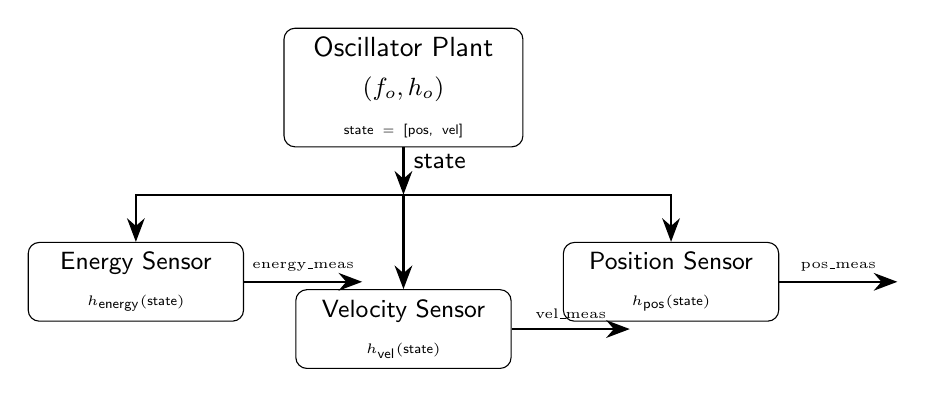
\begin{tikzpicture}[
    node distance=2.5cm,
    block/.style={rectangle, draw, fill=white, text width=2.8cm, text centered, rounded corners, minimum height=1.2cm, font=\sffamily},
    sensor/.style={rectangle, draw, fill=white, text width=2.5cm, text centered, rounded corners, minimum height=1cm, font=\sffamily\small},
    arrow/.style={-{Stealth[length=3mm]}, thick},
    signal/.style={font=\small\sffamily}
]

% Plant block
\node[block] (plant) {Oscillator Plant\\[2pt]{\small $(f_o, h_o)$}\\[2pt]{\tiny state = [pos, vel]}};

% Three sensors
\node[sensor, below right=1.2cm and 0.5cm of plant] (pos_sensor) {Position Sensor\\[2pt]{\tiny $h_{\text{pos}}(\text{state})$}};
\node[sensor, below=1.8cm of plant] (vel_sensor) {Velocity Sensor\\[2pt]{\tiny $h_{\text{vel}}(\text{state})$}};
\node[sensor, below left=1.2cm and 0.5cm of plant] (energy_sensor) {Energy Sensor\\[2pt]{\tiny $h_{\text{energy}}(\text{state})$}};

% Branching point
\coordinate[below=0.6cm of plant] (branch);

% Output coordinates
\coordinate[right=1.5cm of pos_sensor] (pos_out);
\coordinate[right=1.5cm of vel_sensor] (vel_out);
\coordinate[right=1.5cm of energy_sensor] (energy_out);

% Arrows from plant to branch point
\draw[arrow] (plant) -- node[right, signal, pos=0.3] {state} (branch);

% Arrows from branch to sensors
\draw[arrow] (branch) -| (pos_sensor);
\draw[arrow] (branch) -- (vel_sensor);
\draw[arrow] (branch) -| (energy_sensor);

% Arrows from sensors to outputs
\draw[arrow] (pos_sensor) -- node[above, signal, font=\tiny] {pos\_meas} (pos_out);
\draw[arrow] (vel_sensor) -- node[above, signal, font=\tiny] {vel\_meas} (vel_out);
\draw[arrow] (energy_sensor) -- node[above, signal, font=\tiny] {energy\_meas} (energy_out);

\end{tikzpicture}
\end{document}
